\subsection{The actual problem: \textit{aH(t)}}
It all comes down to $aH$ being a decreasing function of time. ($1/aH$ is the \textcolor{darkgreen}{\textit{Hubble radius}})

Use~\eqref{00}~\eqref{continuity} to relate proportionally $a$ and $t$. Then relate $aH$ and $t$, include multiplicative $omega$ factors!. Finally, relate  $aH$ and $a$. 
See that SEC ($\omega>-1/3$) must be violated to have $aH$ increasing. \textcolor{darkred}{$\tau \in \interval[open right]{0}{\infty}$} , violating SEC we can push the singularity to $\tau_i = -\infty$.

%Horizon Problem
\begin{mycolorbox}
    \textbf{Equivalent conditions to $\omega<-1/3$:}

    \begin{enumerate}
        \item Decreasing comoving horizon
        \item Accelerated expansion: $\ddot{a} >0$
        \item Slowly varying $H$ \hfill \textcolor{darkgreen}{$\epsilon_H \equiv -\frac{\dot{H}}{H^2}$}\textcolor{mypurple}{$=3/2 (1+\omega)$} $\quad\Rightarrow \quad\epsilon < 1$
        \item Negative pressure
    \end{enumerate}
\end{mycolorbox}    

\begin{center}
    \begin{tikzpicture}[>=Stealth,thick,x=1cm,y=1cm,font=\small]

        %-------------------------------------------------
        % key coordinates
        %-------------------------------------------------
        \coordinate (tau0)   at (0,4);       % today
        \coordinate (tauEqL) at (0,2);       % τ_eq on axis
        \coordinate (tauEqR) at (2,2);       % τ_eq on light‑cone
        \coordinate (BB)     at (0,-1);      % Big‑Bang (origin of r axis)
        \coordinate (botR)   at (5,-1);      % bottom right on light‑cone
      
        %-------------------------------------------------
        % cyan path CMB
        %-------------------------------------------------
        \path[fill=cyan!20,shade, top color=white,bottom color=cyan!20,line width=1pt]
        (tau0) -- (tauEqR) -- (0,2) -- (tau0) -- cycle;
        \draw[yellow!60!black] (tauEqL) -- (2,0);
        \draw[yellow!60!black] (0,0)     -- (tauEqR); 
        
        %-------------------------------------------------
        % axes
        %-------------------------------------------------
        \draw[->] (0,-1) -- (6,-1) node[below right] {$r$};     % r‑axis
        \draw[->] (0,-1)  -- (0,5) node[left] {$\tau$};        % τ‑axis
      
        %-------------------------------------------------
        % past light‑cone boundary (grey)
        %-------------------------------------------------
        \draw[black,very thick] (tau0) -- (botR);
      
        % dashed horizontal guides
        \draw[dashed] (5,2) -- (0,2) node[left] {$\tau_{rec}$};; 
        \draw[dashed] (5,1.2) -- (0,1.2) node[left] {$\tau_{end}=0$};
        \draw[dashed] (5,-0.25) -- (0,-0.25) node[left] {$\tau_{st}$};
      
        %-------------------------------------------------
        % markers
        %-------------------------------------------------
        \fill (tauEqL) circle (1.5pt);
        \fill (tauEqR)     circle (1.5pt);

        \draw node[left] at (tau0) {$\tau_{now}$};
      
        \draw node[right] at (5,2) {Recombination};

        \draw node[right] at (5,1.2) {Inflation ends};

        \draw node[right] at (5,-0.25) {Inflation starts};
        
        %-------------------------------------------------
        % label boxes
        %-------------------------------------------------
        \node[draw,rounded corners,fill=white,inner sep=2pt]
              at ($(BB)+(1.55,0)$) {BB Singularity};

        \node[draw,rounded corners,fill=cyan!20,shade,
              top color=white,bottom color=cyan!20,inner sep=2pt]
              at ($(tauEqR)+(-1.25,0.35)$) {CMB};

        \node[draw,rounded corners,fill=red!20,shade,
              top color=white,bottom color=red!20,inner sep=2pt]
              at (1.58,-0.1) {Thermalization};   
        
        \node[draw,rounded corners,fill=orange!20,shade,
              top color=white,bottom color=orange!20,inner sep=2pt]
              at (1.14,1.4) {Reheating};       
      
        %-------------------------------------------------
        % τ_i  (inflation era)
        %-------------------------------------------------
        \node[left] at (0,-1) {$\tau_i = -\infty$};
      
      
      \end{tikzpicture}
\end{center}
How much do we need to push back in time $\tau_i$ so that the whole observable universe could have been in causal contact and thus thermalize?

At the onset of inflation assume an universe with far from flat initial conditions: $\Omega_k \sim 1 \Rightarrow \Omega_k(t_{st})/\Omega_k(t_{now})\gg 1$, rewrite and insert $aH(t_{end})/aH(t_{end})$. 
$H$ is nearly constant during inflation, \textcolor{darkgreen}{$N\equiv \log{a}$}. With $\log\left(\frac{a_{end}}{a_{st}}\right)= N_{tot}> 66+ \log{HT^{-1}(t_{end})}$ the flatness problem is solved. Usually, \textcolor{darkred}{\emph{one requires inflation to last 50-60 e-foldings}}.

% Clarifications
\begin{mycolorbox}[blue!30!black]
  
\begin{enumerate}
      \item \textbf{What caused inflation?}
             Whatever it is that drives inflation it must have negative pressure. Thus, it cannot be matter or radiation.
             Neither can be a cosmological constant because it would lead to perpetual rapid inflation (a cosmological constant does not diminish or evolve with time)~\cite{ModernCosm}.
  
             Simplest possibility is via the potential energy of a scalar field $\phi$ (there
             is no known scalar field that can drive inflation). It must have negative pressure and this requirement leads to potential energy dominating over kinetic energy.
      \item \textbf{Why is $H$ const during inflation?} The equation of state for the scalar field gives $\omega \sim -1$. This leads to $H$ being constant. When $\phi$ finishes its roll down the potential, $\omega$ becomes positive and $H$ starts to decrease. This is the end of inflation.
      \item \textbf{Is $a \propto T^{-1}$ valid in every epoch?} It always holds for $T$ being the temperature of radiation. Beware that the latter is not the temperature of the Universe in every epoch.
  \end{enumerate}
\end{mycolorbox}
\begin{figure}[h]
      \centering
      \begin{tikzpicture}
        \node[anchor=south west,inner sep=0] (image) at (0,0) {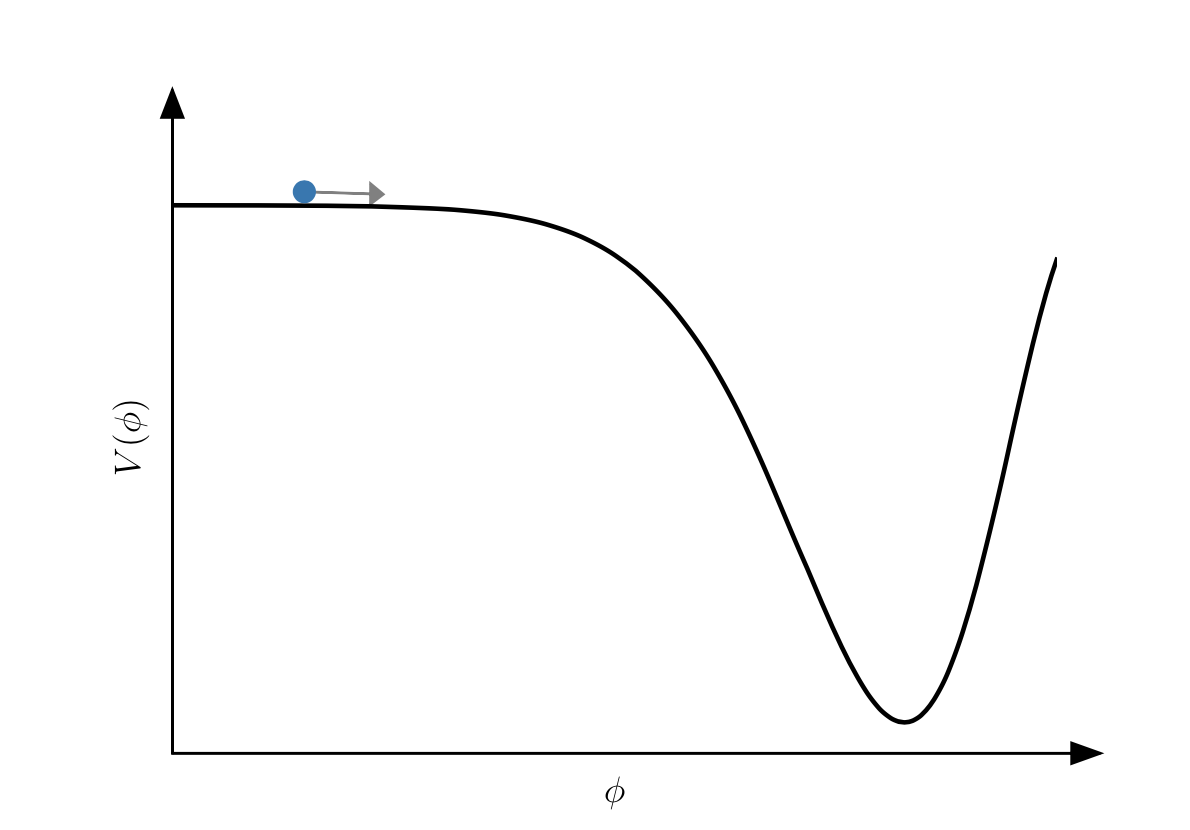
\includegraphics[width=0.8\textwidth]{Graphics/slow-roll.png}};
        \begin{scope}[x={(image.south east)},y={(image.north west)}]
          % Coordinates go from (0,0) bottom-left to (1,1) top-right
          % dashed horizontal guides
          \draw[dashed] (0.76,0.1) -- (0.76,0.8) node[above] {Inflation ends}; 
        \end{scope}
      \end{tikzpicture}
      \caption{A scalr field rolling down a potential~\cite{ModernCosm}.}
  \end{figure}
